\documentclass{article}
\usepackage{ctex}
\usepackage{listings}
\usepackage{xcolor}
\usepackage{pdfpages}
\usepackage{graphicx}

% \usepackage{minted}

\lstset{
	%backgroundcolor=\color{red!50!green!50!blue!50},%代码块背景色为浅灰色
%	rulesepcolor= \color{gray}, %代码块边框颜色
	breaklines=true,  %代码过长则换行
	numbers=left, %行号在左侧显示
	numberstyle= \small,%行号字体
	%keywordstyle= \color{blue},%关键字颜色
	commentstyle=\color{gray}, %注释颜色
%	frame=shadowbox%用方框框住代码块
	frame=single,
	escapeinside=``    % 代码包含中文
}

\begin{document}

\includepdf{cover.pdf}
\section[作业]{作业要求}

\begin{enumerate}
    \item 样本属性可任意输入设定
    \item 先验概率基于训练样本集合自动求得
    \item 混淆矩阵维度可任意设定
\end{enumerate}

\section{实现方案}
\noindent 
csv文件中的训练样本数据支持增删属性,以满足要求1样本属性可任意输入设定。\\
先验概率在BayesClassfier类中实现基于训练样本集合自动求得,满足了要求2。\\
混淆矩阵维度与训练样本数据种类一致,可支持多分类,满足要求3。\\

\noindent
BayesClassifier实现贝叶斯分类的机制如下
\begin{enumerate}
    \item 基于样本训练集计算先验概率
    \item 根据输入的测试数据计算后验概率
    \item 基于后验概率与输入的混淆矩阵计算条件风险
    \item 取条件风险值最小对应的类型实现分类
\end{enumerate}

\section{程序源代码}
\lstinputlisting[language=Python]{../02/bayes_classifier.py}

\section{程序训练数据}

训练样本数据保存在一个csv文件中,由程序进行加载。

\begin{table}[!ht]
    \centering
    \begin{tabular}{|l|l|l|l|l|l|l|l|l|l|}
    \hline
        编号 & 色泽 & 根蒂 & 敲声 & 纹理 & 脐部 & 触感 & 密度 & 含糖率 & 好瓜 \\ \hline
        1 & 青绿 & 蜷缩 & 浊响 & 清晰 & 凹陷 & 硬滑 & 0.697 & 0.46 & 是 \\ \hline
        2 & 乌黑 & 蜷缩 & 沉闷 & 清晰 & 凹陷 & 硬滑 & 0.774 & 0.376 & 是 \\ \hline
        3 & 乌黑 & 蜷缩 & 浊响 & 清晰 & 凹陷 & 硬滑 & 0.634 & 0.264 & 是 \\ \hline
        4 & 青绿 & 蜷缩 & 沉闷 & 清晰 & 凹陷 & 硬滑 & 0.608 & 0.318 & 是 \\ \hline
        5 & 浅白 & 蜷缩 & 浊响 & 清晰 & 凹陷 & 硬滑 & 0.556 & 0.215 & 是 \\ \hline
        6 & 青绿 & 稍蜷 & 浊响 & 清晰 & 稍凹 & 软粘 & 0.403 & 0.237 & 是 \\ \hline
        7 & 乌黑 & 稍蜷 & 浊响 & 稍糊 & 稍凹 & 软粘 & 0.481 & 0.149 & 是 \\ \hline
        8 & 乌黑 & 稍蜷 & 浊响 & 清晰 & 稍凹 & 硬滑 & 0.437 & 0.211 & 是 \\ \hline
        9 & 乌黑 & 稍蜷 & 沉闷 & 稍糊 & 稍凹 & 硬滑 & 0.666 & 0.091 & 否 \\ \hline
        10 & 青绿 & 硬挺 & 清脆 & 清晰 & 平坦 & 软粘 & 0.243 & 0.267 & 否 \\ \hline
        11 & 浅白 & 硬挺 & 清脆 & 模糊 & 平坦 & 硬滑 & 0.245 & 0.057 & 否 \\ \hline
        12 & 浅白 & 蜷缩 & 浊响 & 模糊 & 平坦 & 软粘 & 0.343 & 0.099 & 否 \\ \hline
        13 & 青绿 & 稍蜷 & 浊响 & 稍糊 & 凹陷 & 硬滑 & 0.639 & 0.161 & 否 \\ \hline
        14 & 浅白 & 稍蜷 & 沉闷 & 稍糊 & 凹陷 & 硬滑 & 0.657 & 0.198 & 否 \\ \hline
        15 & 乌黑 & 稍蜷 & 浊响 & 清晰 & 稍凹 & 软粘 & 0.36 & 0.37 & 否 \\ \hline
        16 & 浅白 & 蜷缩 & 浊响 & 模糊 & 平坦 & 硬滑 & 0.593 & 0.042 & 否 \\ \hline
        17 & 青绿 & 蜷缩 & 沉闷 & 稍糊 & 稍凹 & 硬滑 & 0.719 & 0.103 & 否 \\ \hline
    \end{tabular}
\end{table}

\section{程序运行结果}

% \begin{figure}[H] %H为当前位置,!htb为忽略美学标准,htbp为浮动图形
%     \centering %图片居中
%     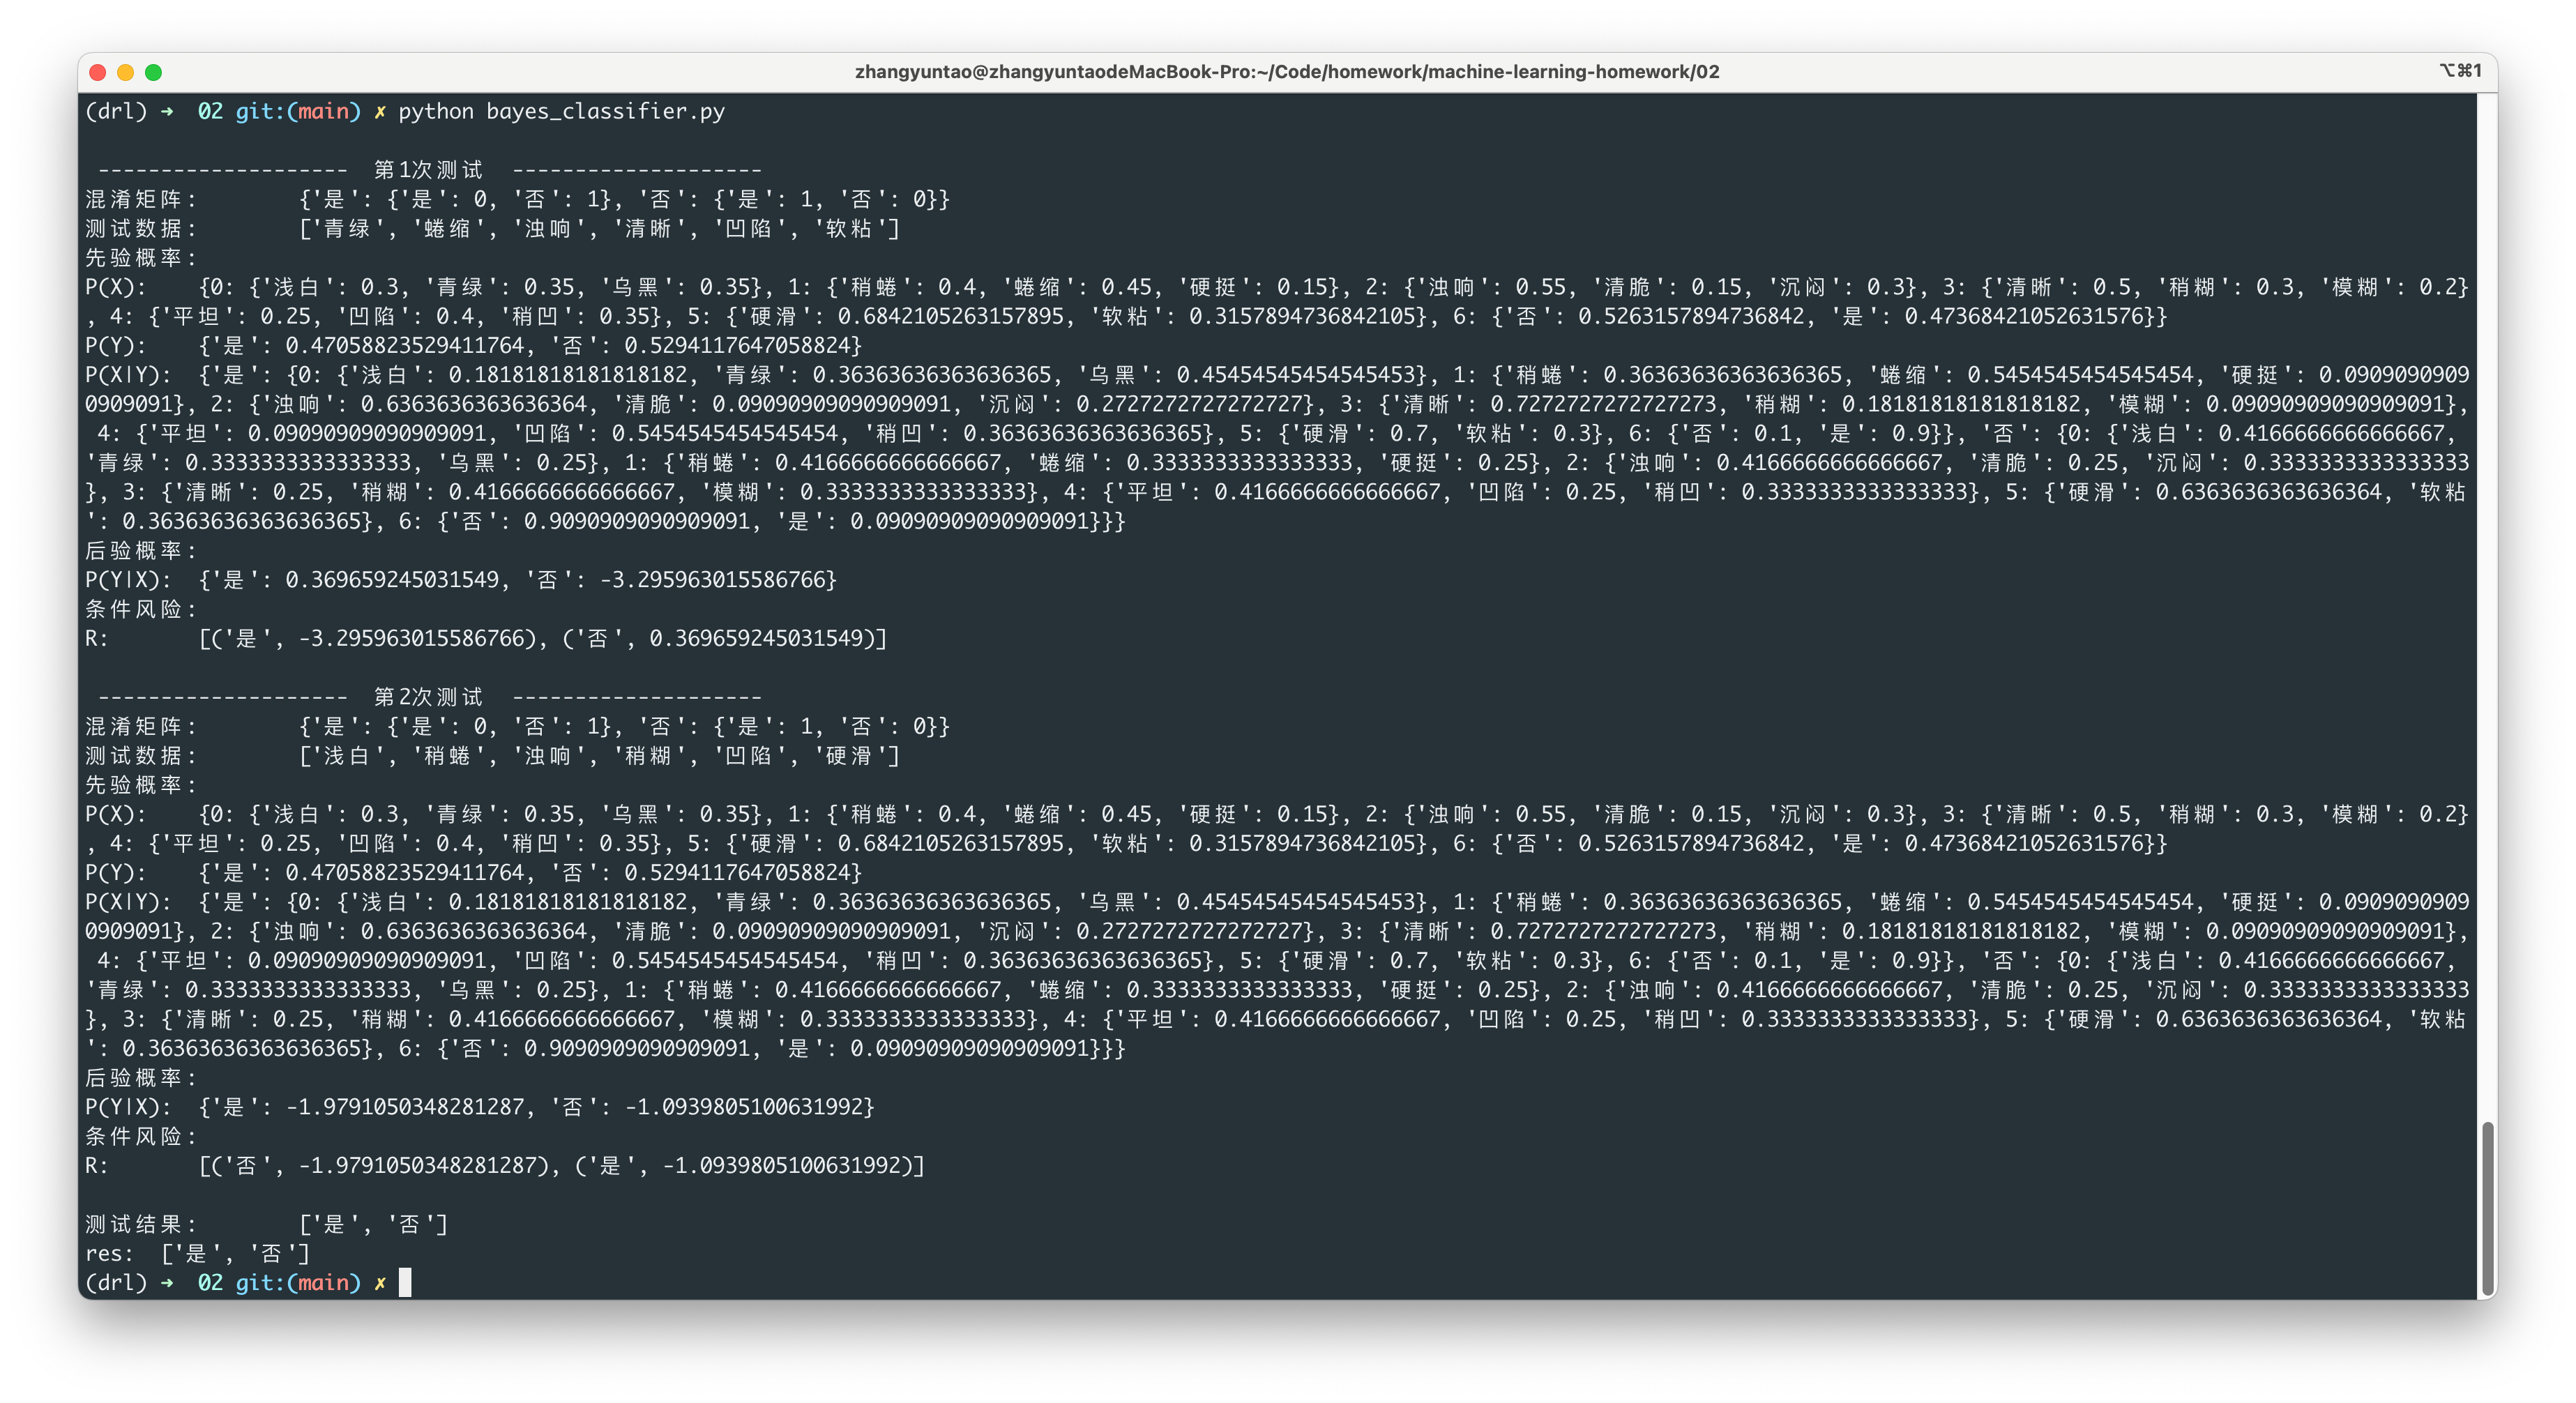
\includegraphics[width=0.7\textwidth]{bayes_exec_res.png} %插入图片,[]中设置图片大小,{}中是图片文件名
%     \caption{Main name 2} %最终文档中希望显示的图片标题
%     \label{Fig.main2} %用于文内引用的标签
% \end{figure}




\end{document}